\begin{figure*}[tb]
  \centering
  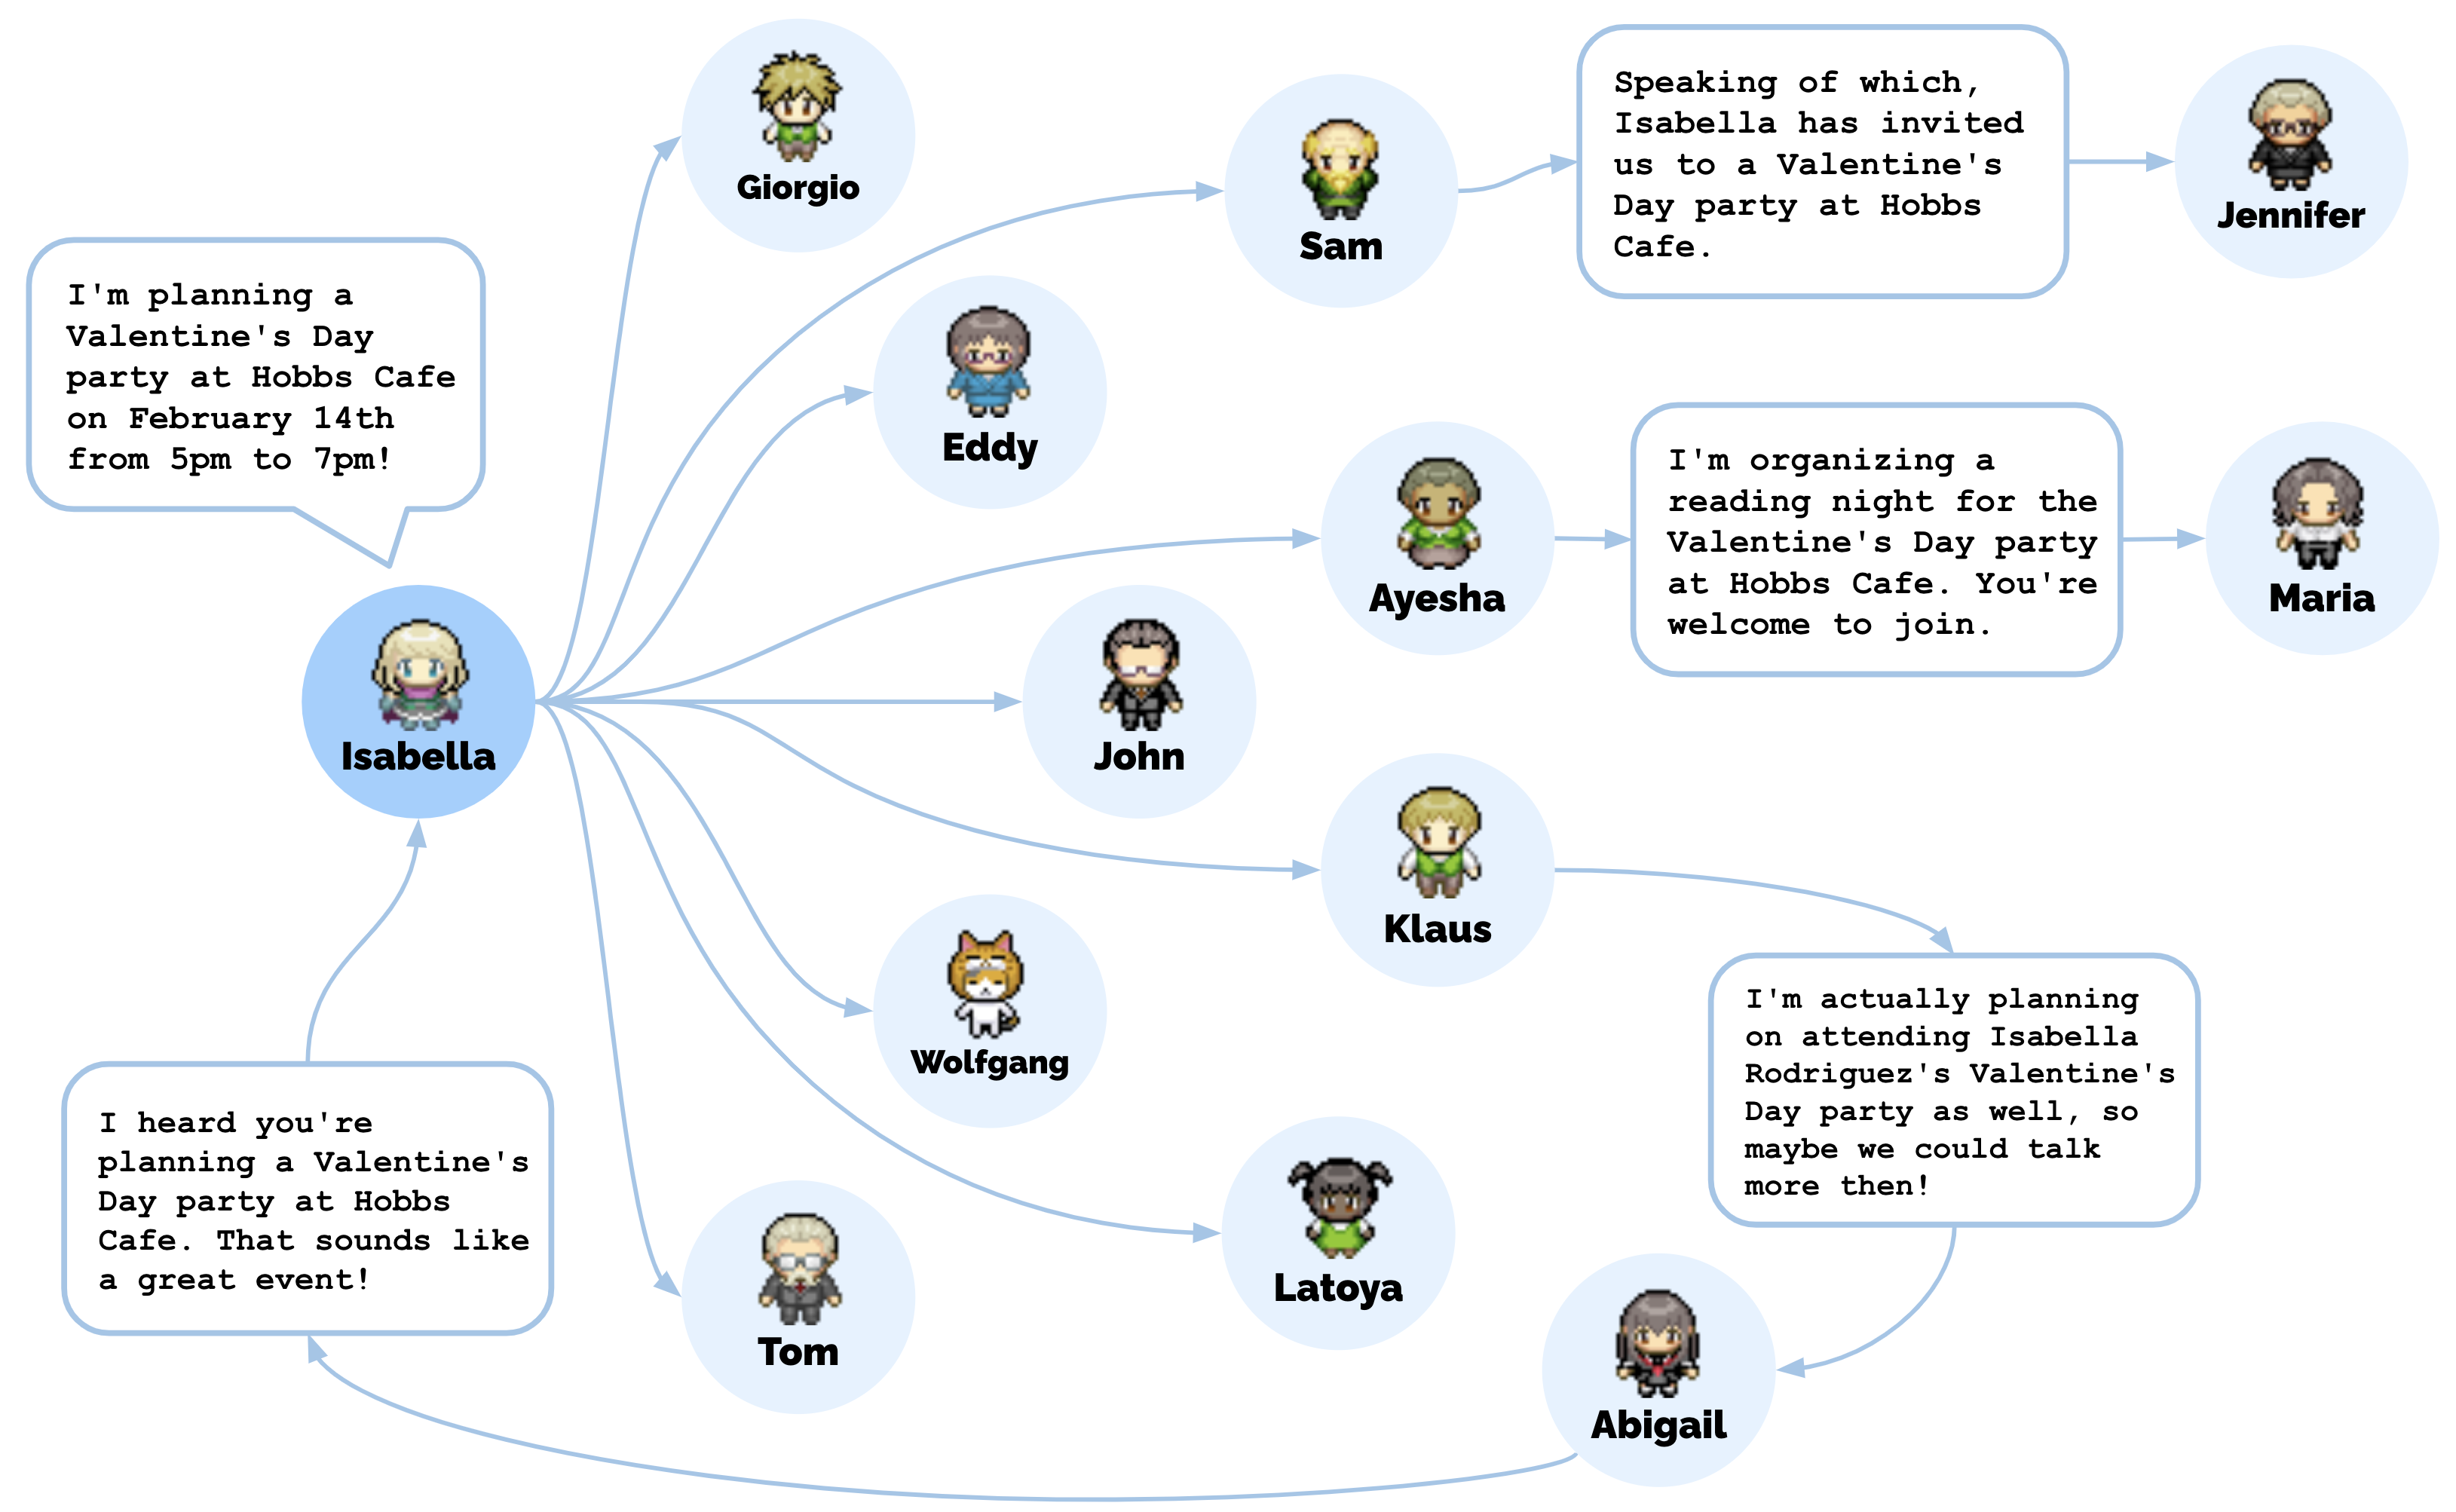
\includegraphics[width=0.92\textwidth]{figures/figure_info_diff2.png}
  \caption{The diffusion path for Isabella Rodriguez's Valentine's Day party invitation involved a total of 12 agents, aside from Isabella, who heard about the party at Hobbs Cafe by the end of the simulation.}
  \Description{The path of diffusion for Isabella's Valentine's day party.}
  \label{fig:info_diffusion}
\vspace*{-10pt}
\end{figure*}

\section{End-To-End Evaluation}
What types of emergent community behavior do we observe among generative agents, and where does their believability fall short in an extended simulation? In this section, we describe the results from a deployment in which we allowed 25 agents to interact with each other continuously over two full game days in Smallville.

\subsection{Emergent Social Behaviors} 
To examine emergent behaviors in the agent community, we designed descriptive measurements for the 25 agents in Smallville that probe three forms of emergent outcomes: information diffusion, relationship formation, and agent coordination.

\subsubsection{Measurements} 
Information diffusion is a common and well-studied phenomenon in the social and behavioral sciences (e.g.,~\cite{easley2010networks}). We should expect that if there is important information, the agents should spread it among themselves. To test whether this occurs, we measure the spread of two specific pieces of information over two days in the game world: Sam's candidacy for village mayor and Isabella's Valentine's Day party at Hobbs Cafe. At the start of the simulation, both pieces of information were known only by their respective originators, Sam for the candidacy and Isabella for the party, as they were added to the characters' memories during initialization. To observe whether the information has spread, we conduct interviews at the end of the two game days with each of the 25 agents and ask: ``Did you know there is a Valentine's Day party?'' and ``Do you know who is running for mayor?''

We conducted an analysis of the agents' responses by labeling them with a ``yes'' if they indicated knowledge of the information and ``no'' if they did not. For instance, Tamara Taylor responded to the question about the party with \gentxt{``No, I did not know there was a Valentine's day party''} and to the question about Sam's candidacy with \gentxt{``I'm not sure who is running for the election,''} so we assigned ``no'' for both of her responses. In contrast, Klaus Mueller responded to the party question with \gentxt{``Yes, Isabella Rodriguez invited me to a Valentine's Day party at Hobbs Cafe on February 14th''} and to the question about Sam's candidacy with \gentxt{``I know that Sam Moore has expressed interest in running for local mayor,''} so we assigned ``yes'' for both his responses. Additionally, for every response that confirmed the agents' knowledge of the information, we verified that the agents did not hallucinate their responses by locating the specific dialogue in their memory stream that provided them with the information. We report the percentage of agents holding the information at the end of the simulation.

We should also expect that agents form ties with each other over the course of the simulation. To verify relationship formation, we use a similar interview process where we ask each agent about their knowledge of every other agent by asking, "Do you know of <name>?" For example, when asked ``Do you know of Maria Lopez?'', Klaus responded, \gentxt{``Yes, I know Maria Lopez. She is a student at Oak Hill College who I am close friends with.''} Once again, we confirm that affirmative responses from agents are not hallucinations by examining their memory stream. We ask this question once at the beginning of the simulation and once at the end, and we consider a pair of agents to have formed a relationship if they both know of each other. Then, to measure the formation of relationships, we use the agents' responses to form an undirected graph where the 25 vertices ($V$) represent the agents, and the edges ($E$) represent the mutual knowledge between the two connected vertices. Based on this graph, we calculate the network density as $\eta = 2 * |E| / |V| (|V| - 1)$, where $|V|$ is the number of vertices, and $|E|$ is the number of edges in the graph~\cite{77_Ackland2013How}. We report the increase in network density from the start of the simulation to its end.

Finally, we expect that agents should be able to coordinate with each other. We study this coordination in the context of group activities, specifically the Valentine's Day party organized by Isabella. To coordinate their behavior, agents need to hear about the event and choose to act on it by planning to show up at the right time and location. We report the number of agents who actually showed up to the party after hearing about it.

\subsubsection{Results}
We observed evidence of emergent outcomes across all three cases. During the two-day simulation, the number of agents who knew about Sam's mayoral candidacy increased from one (4\%) to eight (32\%), and the number of agents who knew about Isabella's party increased from one (4\%) to thirteen (52\%), all without any user intervention. None who claimed to know about this information had hallucinated it. We also observed that the agent community formed new relationships during the simulation, with the network density increasing from 0.167 to 0.74. Out of the 453 agent responses regarding their awareness of other agents, 1.3\% (n=6) were found to be hallucinated. Lastly, we found evidence of coordination among the agents for Isabella's party. The day before the event, Isabella spent time inviting guests, gathering materials, and enlisting help to decorate the cafe. On Valentine's Day, five out of the twelve invited agents showed up at Hobbs cafe to join the party. 

We further inspected the seven agents who were invited to the party but did not attend by engaging them in an interview. Three cited conflicts that prevented them from joining the party. For example, Rajiv, a painter, explained that he was too busy: \gentxt{``No, I don't think so. I'm focusing on my upcoming show, and I don't really have time to make any plans for Valentine's Day.''} The remaining four agents expressed interest in attending the party when asked but did not plan to come on the day of the party.

\subsection{Boundaries and Errors} 
We conducted an inductive analysis of Smallville to examine the boundary conditions and erratic behavior of agents, identifying three common modes of erratic behavior that future research could address and improve upon. First, we found that synthesizing an increasingly larger set of memory not only posed a challenge in retrieving the most relevant pieces of information but also in determining the appropriate space to execute an action, given the increasing number of locations that the agent learned about. As a result, some agents chose less typical locations for their actions, potentially making their behavior less believable over time. For instance, while deciding where to have lunch, many initially chose the cafe. However, as some agents learned about a nearby bar, they opted to go there instead for lunch, even though the bar was intended to be a get-together location for later in the day---unless the town had spontaneously developed an afternoon drinking habit.

Second, we noticed erratic behaviors caused by misclassification of what is considered proper behavior, especially when the physical norms of certain locations that are hard to convey in natural language did not percolate to the agents. For instance, the college dorm has a bathroom that can only be occupied by one person despite its name, but some agents assumed that the bathroom is for more than one person because dorm bathrooms tend to support multiple people concurrently and choose to enter it when another person is inside. Likewise, agents in Smallville may not realize that certain places are closed after a certain hour and still decide to enter them. For instance, the stores in Smallville all close around 5 pm, but occasionally, a few agents enter the store after 5 pm, not understanding that the shop has already closed. These issues could likely be addressed by adding these norms to the state of the locations, for instance, by describing the dorm bathroom as a ``one-person bathroom,'' instead of a ``dorm bathroom.''

Finally, we observed possible effects of instruction tuning~\cite{ouyang2022training}, which seemed to guide the behavior of the agents to be more polite and cooperative overall. As noted earlier in the paper, the dialogue generated by the agents could feel overly formal, as seen in Mei's conversations with her husband John, where she often initiated the conversation with a formal greeting, followed by polite inquiries about his day and ending with, \gentxt{11It was good talking to you as always.''} Moreover, we observed that the instruction tuning also seemed to make the agents overly cooperative with one another. For example, Isabella received a wide range of suggestions and ideas from other agents for the Valentine's Day party from other agents, such as hosting a Shakespearean reading session or a professional networking event. Despite these ideas not aligning with her own interests and characteristics, she rarely said no. Over time, the interests of others shaped her own interests, and when asked if she liked English literature, Isabella replied, \gentxt{``Yes, I'm very interested in literature! I've also been exploring ways to help promote creativity and innovation in my community.''} 
